%%%%%%%%%%%%%%%%%%%%%%%%%%%%%%%%%%%%%%%%%%%%%%%%%%%%%%%%%%%%%%%%%%%%%%%%%%%%%%%%
%2345678901234567890123456789012345678901234567890123456789012345678901234567890
%        1         2         3         4         5         6         7         8

\documentclass[letterpaper, 10 pt, conference]{ieeeconf}  % Comment this line out
                                                          % if you need a4paper
%\documentclass[a4paper, 10pt, conference]{ieeeconf}      % Use this line for a4
                                                          % paper

\IEEEoverridecommandlockouts                              % This command is only
                                                          % needed if you want to
                                                          % use the \thanks command
\overrideIEEEmargins
% See the \addtolength command later in the file to balance the column lengths
% on the last page of the document



% The following packages can be found on http:\\www.ctan.org
\usepackage{graphics} % for pdf, bitmapped graphics files
\usepackage{caption}
\usepackage{subcaption}
\usepackage{epsfig} % for postscript graphics files
\usepackage{mathptmx} % assumes new font selection scheme installed
\usepackage{times} % assumes new font selection scheme installed
\usepackage{amsmath} % assumes amsmath package installed
\usepackage{amssymb}  % assumes amsmath package installed

\title{\LARGE \bf
Interception of moving objects with a robotic arm in a simulated environment
}

\author{Juan Garcia, Harrison Jones and Arash Rouhani*
  \thanks{\texttt{*\{jgarcia39,harrisonhjones,rarash\}@gatech.edu}}
}


\begin{document}

\maketitle
\thispagestyle{empty}
\pagestyle{empty}


%%%%%%%%%%%%%%%%%%%%%%%%%%%%%%%%%%%%%%%%%%%%%%%%%%%%%%%%%%%%%%%%%%%%%%%%%%%%%%%%
\begin{abstract}

The problem of catching a moving object can be divided into two sub problems.
First, the object must be perceived and its path must be estimated in order for
movements to be calculated that would result in successfully catching the
object in the future. The second sub-problem is to find a catching
configuration. This paper focuses primarily on the second problem of finding an
acceptable configuration. Simple models that simulate sensor inaccuracy and
randomness are used to closely simulate real environments, and regression
models are used to estimate the object's path in these simulated real
environments. Since multiple end configurations are acceptable as the goal, we
introduce a new concept called a multi-goal RRT, a modified version of
Rapidly-exploring Random Trees (RRTs), which grows towards multiple goals
simultaneously. This approach was implemented in an attempt to have the RRT
grow toward several predicted path nodes. The multi-goal RRT was compared
against a regular RRT. The results show promise for the application of
Multi-goal in a real-world setting.

\end{abstract}

%%%%%%%%%%%%%%%%%%%%%%%%%%%%%%%%%%%%%%%%%%%%%%%%%%%%%%%%%%%%%%%%%%%%%%%%%%%%%%%%
\section{INTRODUCTION}

\subsection{Motivation}

Robots will need to successfully intercept and catch moving objects as their
abilities become more acquainted for daily human use. The applications of such
ability range from military to assistive operations in the home. Robotic agents
able to track and intercept moving objects constitute a valuable military
asset, as they could provide protection and tactical superiority to ground
troops through the stoppage of missiles, grenades and harmful projectiles.
Flying-drones would enhance their current capabilities, as they would be able
to automatically track objects of interest and intercept enemy projectiles
aimed at larger vehicles with human personnel.  Tracking and interception
abilities also have an application in the Biology and Genetics fields as
researchers could benefit from automated counting and transporting of live
cells, essential operations in many cellular engineering applications such as
cell sorting and fusion \cite{5985660}. An ability to catch moving objects
would also be beneficial in the field of Socially Assistive Robotics (SAR), as
the main objective is to stimulate the rehabilitation and management of
lifelong cognitive, social and physical disorders \cite{5569021}. Robotic
agents could motivate patients to lift objects as part of their training and
rehabilitation, serving as playmate for ball throwing, object lifting and tool
handling exercises. In addition, robots could monitor patient's progress in
order to catch drop objects and avoid injuries.

We were specifically motivated to pursue this project by two ideas. One is a
video that illustrates a robot capable of ”catching” a piece of trash thrown
using a vision system and limited path planning. The little trash robot seemed
pretty interesting and useful, and initially the thought of expanding on the
idea was toyed with. The other source of motivation came from a previous piece
of work performed under Professor Mike Stilman at Georgia Institute of
Technology. Tobias Kunz had worked on an algorithm that blocked known sword
paths in a simulated environment \cite{lampariello2011trajectory}. The group
had not explored the idea of predicting a sword swing given the current path of
the sword.

\subsection{Problem}

Given the explained motivations, we defined the problem to be tackled as the
interception of a moving object using a 7 DOF robotic arm in a noisy simulated
environment with limited information on the objects’ path. The object in our
case would be a moving sphere that is allowed to go through obstacles as it
follows its calculated projectile path. The arm is not allowed to hit any
obstacles as it tries to catch as many sequential spheres as possible, with an
increasing amount of sensor and environment simulated noise.

\subsection{Solution}

The solution described in this paper utilizes an algorithm which tracks the
object, predicts its future path, and then moves a virtual robot arm to
intercept it. This is done by using two different prediction
algorithms, a linear predictor, used for straight motions such as punching, and a
quadratic predictor, used for projectile objects such as thrown trash or balls. After
computing a predicted path, a Multi-goal RRT is used to move the robot arm to
intercept the object while still avoiding obstacles in its environment.



\section{RELATED WORK}

The problem of tracking and intercepting moving objects with robotic agents has
been a well-researched topic through the combination of Computer Vision,
Planning and Machine Learning techniques. As there have been many previous efforts to intercept moving objects,
we will list key results that provide insights into the challenges of such
endeavor. Peter Allen et al. at the University of Columbia utilized optic-flow
techniques to track a moving object in a circular track with a PUMA robotic
arm. Most importantly, they separated the perceived coordinates into a XY plane
and a Z-axis, modeled motion through derivations of velocity and curvature, and
ran a developed filtering method to handle noise sources and estimate arc and
bending characteristics \cite{Allen91automatedtracking}. Their results
showcased a robust enough method able to repeatedly pick up an object moving in
a planar surface and grasp it.  More recently, Jens Kober et al. at Disney
Research developed tracking and prediction methods to allow a robot to play
catch and juggle a ball \cite{koberplaying}. In their approach, they utilized
Hough-transforms to track the moving balls through an external camera system.
For prediction, they modeled the balls’ motion as point masses (i.e. quadratic
predictors) and implemented Kalman filters for handling noise and environment
uncertainties. The results obtained showed a potential for having safe
human-interactive robotic characters throughout theme parks, but much work was
still needed in order to increase the robot's reachable area and degrees of
freedom, both constrained during experimentation in order to facilitate the
approach. To tackle catching objects with robots in real-time, Jan Peters et
al. proposed in \cite{lampariello2011trajectory} the formulation of a
non-linear constrained-optimization problem where the desired trajectories are
encoded through parametric representation. The result of such optimization is
then used through Nearest Neighbor, Support Vector Machines and Gaussian
regression to allow a real-time execution. Their results showcases the
trade-offs between computational time and accuracy for real-time operations, as
accuracy in prediction must be satisfied in order for the robot to be able to
catch the moving object. In this project, we wish to explore the initial
feasibility of using RRTs variants for intercepting moving objects in a
simulated environment. Although RRTs have been extensively used in the planning
domains, no relevant previous work was found where such technique was
specifically used for object interception.

\section{METHODS}

We'll cover the methods in the order they are used in a complete simulation.
First, we must generate a projectile path, then distortion is applied. In order
to know where it's possible to catch the object some path prediction is used.
Then to actually get a series of possible robot stances, inverse kinematics is
applied to get some corresponding joint configuration for each projectile
position. Finally, and most highlighted part in this paper, we search for the
easiest to reach joint space configuration. It should be noted that this whole
process is done iteratively, as at fixed time steps we replan taking into account
the most recent observation of the projectile.

\subsection{Path Projection}

We create a path by sampling positions from the formula for projectile motion:

\[
  \vec{x}(t) = \vec{x}_0 + \vec{v}t + {\vec{a}t^2 \over 2}
\]

Where the arrow notation denotes a variable being a vector in the
workspace.  This simple equation covers most of the motions in our
application except for wind resistance. Note that by setting the
acceleration to $\vec{0}$ the projectile will be a straight line
resembling a straight punch. By setting $\vec{a} = -\vec{g}$ where
$\vec{g}$ is a gravity constant we get a standard "shoot from canon"
projectile motion. Wind is simulated by adding a random constant to
the acceleration.

\subsubsection{Deciding $\vec{x}$, $\vec{v}$ and $\vec{a}$}

We just saw how changing the acceleration we'll get simple models of
different behaviors that might be desired for our intended application.
However, in all cases we must make sure that it will be possible at all
to catch the thrown object, in other words, the trajectory must
intersect the set of reachable points of the arm. To ensure that we
introduce two new points, a \emph{random start position}, that simply is
$\vec{x}_0$ and a \emph{random reachable position} which is a random
point reachable by the robot arm. With these approach in mind one can
solve for the velocity if we fix the acceleration. To simplify further
and decrease the solution space we set that the velocity to have an
angle of 45 degrees from the floor plane. For the wind to actually have
a negative impact, we let the calculations of the velocity be oblivious
of it.

\subsubsection{Distortion}

Since in later steps of the iteration the robot is going to predict the
remaining path, we must add distortion to it to make it impossible to
retrieve the whole original exact path again. It's hard to motivate
any model besides simple randomness here.

\[
  \vec{x}_{observed}(t) = \vec{x}(t) + noise
\]

Where for each discrete time step in our simulation the $noise$ is a vector
where each coordinate is a uniform distribution in $[-\mu, \mu]$

\subsection{Path Prediction}

Given some sample points, we work backwards from the equations in the
model for path projection.  We have two prediction models, one assumes
straight motion and the other projectile motion.  The equation

\[
  \vec{x}_{observed}(t) = \vec{x}_0 + \vec{v}t + {\vec{a}t^2 \over 2}
\]

will cover both cases, only that you set $a=0$ in the linear version.
However, only two and three data points are required to solve this
system for the linear and quadratic version respectively, to fix that we
simply only look at the most recent data points we require.

Note that this is of course not exact as  it does not compensate for the
unknown noise, to compensate for the noise, one can treat a chunk of
points  as one point by taking their average. Note that with this
strategy we still need more points for the quadratic version. If the
chunk sizes are to small, we won't defeat noise and if it's too small we
won't be able to estimate the trajectory, as we must wait until we have
enough points to create the chunks. Therefor a dynamic chunk size was
chosen that grows with number of data points. A cap was set on the chunk
size to avoid looking at too old and outdated data.

We found both the working backwards from the equations prediction and
the idea of chunking the data to be the simplest to implement and choose
that over more sophisticated regression.

\subsection{Inverse kinematics}

Knowing the trajectory, one can use inverse kinematics to find a corresponding
joint space configuration. We do use the pseudo inverse Jacobian method.
That is to simply iterate

\[
  \Delta q = \mathbf{J}^{+} \Delta x
\]

until convergence where $\mathbf{J}^{+} =
\mathbf{J}^T(\mathbf{J}\mathbf{J}^T)^{-1}$.


\subsection{Planning}

We plan with either one of the two algorithms, the regular RRT
\cite{lavalle2001randomized} and the multi-goal RRT that is introduced in this
paper. Which of the two we use will depend on the parameters we set before we
start a single simulation.

The multi goal RRT is working very much like the traditional one with
the exception that there are multiple goals and reaching any one of them
is considered a success. One might think of two different strategies for
the multi goal RRT. The first being that you return the first path that
leads to any of the goals and the second strategy is to make sure you've
got a path for each goal and then return the shortest. The first one is
always faster because it don't need to grow the tree until each goal has
been reached. Since it also was simpler to implement we went with a
multi goal RRT using the first strategy.

What differs between a regular RRT and any of the two multi goal RRTs
kinds is only the termination condition. The single RRT continues to
grow until the goal has been reached, the first strategy of the multi
goal keeps growing until \emph{any} goal has been reached while the
other strategy keeps growing the tree until \emph{all} goals have been
reached.

As for the concepts of greedy, connect and bidirectional, only greedy and the
connect strategy is applicable to the multi goal RRT. The original greedy
strategy takes the goal and grows towards it\cite{robocup, FergusonKS06}. In
our case we take any of the goals randomly and grow towards it. As for connect
one would imagine growing towards a random configuration and then keep growing
to the same configuration until one collides, just like the original connect
algorithm does\cite{kuffner2000rrt}. We will, however, only use the greedy goal
biasing in both our regular RRT implementation and multi-goal RRT. The reason
for this was to make the behavior easier to reason about than it would be if
multiple features could cause unexpected results.

% We consider the connect strategy to defeat the purpose of the
% multi goal rrt, as if we have an extreme case where there are no objects to
% block the path, connect would just randomly pick any of the goals and keep
% growing to it and the purpose of choosing the goal with the closest distance
% with respect to objects is defeated.

\subsection{Replanning, Discretization and Arm Speed}

Before one iteration is done and we start replanning with the most recently
observed data we move the arm. For the simulation to be realistic, the  maximum
distance the arm can move must be limited for each time step. The question is
how distance is measured, or rather in which norm. Most realistically for our
application might have been the infinity norm, which means that all joints are
allowed to rotate a fixed amount of degrees independent of each other.
Regardless of that we used regular euclidean distance, the two norm. The reason
is that we set the step size parameter to the RRT and interpret the second
position in its returned path as the next position for the arm.

With the joints configured to their new angles, we increase the
simulation time by the fixed $\Delta t$ and keep iterating and replan as
we allow our path predictor is fed with more points in the observed trajectory.

\section{EXPERIMENTS}

The experimentation and accompanied development were targeted towards (1)
determining the robustness of the approaches presented to noise sources and (2)
selecting the best combination of predictors and RRT-variants for use in a
future non-simulated setting. The overall approach presented in the previous
sections was tested in the DART/GRIP environment through a developed interface
that allowed for the specification of different amounts of noise, number of
simulations, predictor type, among other parameters.  The results were analyzed
according to the following criteria: (i) success rate given an amount of noise,
(ii) success rate vs. increasing amounts of noise for different combinations of
RRT-variants and predictors, (iii) completion time given an amount of noise.
Success rate was defined as the amount of times the arm was able to intercept
the moving sphere divided by the total number of simulations (i.e. a
percentage). The workspace distance $d$ between the arm's end-effector and the
moving sphere was repeatedly calculated in order to determine whether an
interception had occurred. If $d$ was less than a given threshold $t$, then the arm
successfully intercepted the moving sphere. In this case, $t$ was set to the
radius of the sphere (i.e. 0.12).  The graphs shown below summarize the results
of the experiments undertaken. Their connotations and insights will be analyzed
in the following section.

\section{ANALYSIS}

\begin{figure}
        \centering
        \begin{subfigure}[b]{0.5\textwidth}
                \centering
                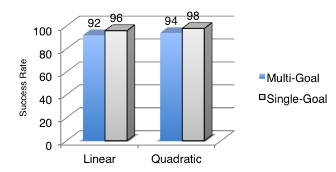
\includegraphics[width=\textwidth]{fig/noise-005}
                \caption{$\mu = 0.05$}
                \label{fig:noise-005}
        \end{subfigure}%
        \\
        ~ %add desired spacing between images, e. g. ~, \quad, \qquad etc. 
          %(or a blank line to force the subfigure onto a new line)
        \begin{subfigure}[b]{0.5\textwidth}
                \centering
                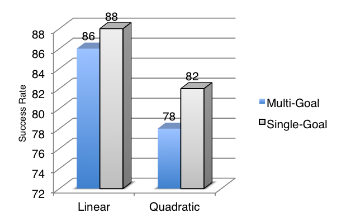
\includegraphics[width=\textwidth]{fig/noise-009}
                \caption{$\mu = 0.09$}
                \label{fig:noise-009}
        \end{subfigure}
        ~ %add desired spacing between images, e. g. ~, \quad, \qquad etc. 
          %(or a blank line to force the subfigure onto a new line)
        \caption{Success rates for combinations of Multi-Goal RRT, Single-RRT, Linear and Quadratic predictors after 100 simulations having varying noise $\mu$}\label{fig:noise}
\end{figure}

Figure \ref{fig:noise-005} shows the success rates for combinations of
Multi-goal and Single-goal with Linear and Quadratic predictors after
100 simulations with a noise of 0.05. In both cases, the Single-goal
approach achieves a higher success rate than the Multi-goal approach.
The difference in such success, an average of 3 percent units, is not
enough to conclude the dominance of one method over the other for this
given noise amount. In addition, the quadratic predictor seems to yield
higher success rates when used by both approaches with this noise
amount, indicating the better representation of the projectile path by
our predicting equations.

Figure \ref{fig:noise-009} , in contrast, showcases a much more
interesting scenario. With a noise amount of 0.09, the Multi-goal and
Single-goal approaches achieve similar success rates (about 87 percent)
when employing the Linear predictor. When the approaches utilize the
Quadratic predictors their success rates drop by a combined average of 8
percent units. In this case, the Multi-goal approach achieves a
noticeably lower success rate. With a significant increase in sensor
noise, the robotic arm's perceived sphere path does not longer follow
projectile motion characteristics as the sphere bounces around. In this
case, the Quadratic predictor in a way over fits the model as it uses 3
averaging points to predict a curved motion. The Linear predictor only
predicts line trajectories that with a clutter of perceived points yield
higher accuracy rates.

\begin{figure}
        \centering
        \begin{subfigure}[b]{0.22\textwidth}
                \centering
                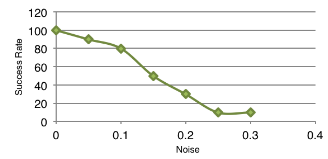
\includegraphics[width=\textwidth]{fig/multi}
                \caption{Multi goal RRT}
                \label{fig:multi}
        \end{subfigure}%
        ~ %add desired spacing between images, e. g. ~, \quad, \qquad etc. 
          %(or a blank line to force the subfigure onto a new line)
        \begin{subfigure}[b]{0.24\textwidth}
                \centering
                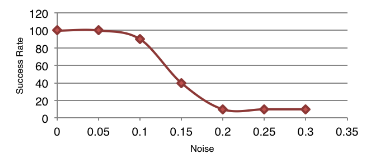
\includegraphics[width=\textwidth]{fig/single}
                \caption{Single goal RRT}
                \label{fig:single}
        \end{subfigure}
        ~ %add desired spacing between images, e. g. ~, \quad, \qquad etc. 
          %(or a blank line to force the subfigure onto a new line)
        \caption{Average RRT success rates versus increasing noise
        with Linear Predictor; 10 simulations for each increase in 0.05
      noise}\label{fig:rrts}
\end{figure}

Figure \ref{fig:rrts} depict the performance of both the Single-goal and
Multi-goal RRT approaches as the noise amount increases. A Linear
predictor was utilized in both cases as previous analysis demonstrated
its robustness to sensor noise. For each noise case, the average success
rate of 10 simulations was computed. Both approaches’ rates steadily
drop as the amount of noise increases, with the Single-goal RRT staying
above 90\% for noise sources between 0 and 0.1 while the Multi-goal RRT
only for value between 0 and 0.05. The similar behavior of both
approaches regarding an increase in noise showcases the need to
implement better prediction techniques, as the current ones are only
naive approaches to tackle such noise and uncertainty scenarios. A more
thorough analysis of these approaches’ response in noisy situations
would be achieved through known regression and estimation techniques.
Time constraints forced these topics to be considered for future work.

\begin{figure}
        \centering
        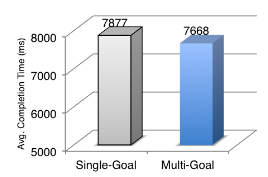
\includegraphics[width=3in]{fig/runtimes}
        \caption{Average times for Single-goal and
        Multi-goal RRTs after 100 simulations with both Linear and
      Quadratic predictors where $\mu = 0.05$}\label{fig:runtimes}
\end{figure}

At last, Figure \ref{fig:runtimes} presents the average execution times
during 100 simulations of Single-goal and Multi-goal RRTs with Linear
predictors. Multi-goal RRTs achieve faster execution times (i.e. 200ms
difference) than Single-goal RRTs as the tree growth is biased by all
reachable points of the sphere trajectories. When any goal is reached,
reaching the rest is not computationally expensive as these points are
expected to be mostly close in space and time. Single-goal RRTs in
contrast, constantly expands the tree towards the closest point in terms
of joint space distance, thus taking longer to get there.



We examined projectile path's through passing reachable areas surrounded
with obstacles to determine the qualitative difference between the RRT
kinds. Figure \ref{fig:visrrts} shows two resulting configurations for
Multi-goal and Single-goal RRTs given the same projectile path. Above
80\% of the time, the Multi-goal RRT choose to catch the object before it
collided with the object, while Single-goal RRT usually waited for the
object in the later parts of the motion. We believe such behavior is due
to the fact that the Single-goal RRT picks the closest point in terms of
joint space distance and in this case, such point is located in the
space after the sphere passes through the obstacle. In a sense,
Single-goal RRT is a lazy approach, as it will try to intercept the
moving sphere with the minimum joint effort possible. On the other hand,
Multi-goal RRT considers all points in the reachable object trajectory,
and when any of them is reached, it returns a path to follow. This
implementation generally tries to catch objects at earlier times as this
allows for some leniency in terms of replanning if its not able to catch
the moving sphere.

\section{DISCUSSION}

It would be interesting to test the algorithms in an environment where
there are more objects that the arm can't touch. Such experiments might
lift the potential from multi goal RRTs,  if a multi goal RRT should
prove useful against the single goal RRT aimed at the closest goal, it
must expand a towards a more distant goal which in fact is closer with
respect to there being objects in the way for reaching the close goal.
While there might be many factors for the results for figure
\ref{fig:runtimes}, one might guess that the approximately equal
run times was due to that they reached their goal in the same amount of
steps and that is because the closest goal without respect to object was
the same goal with respect to objects. On the other hand then one might
expect their performance over all be quite similar which it appears not
to be from figure \ref{fig:noise} and \ref{fig:rrts}, maybe it's
decrease in performance was simply due to it usually founds the same
closest object but occasionally in between the iterations detours to
another goal making it somewhat more clumsy.

Another idea stemming from the discussion above is to not actually do
replanning, since the nature of randomness in the RRT makes it non optimal
and it would be better to committing to trying to reach one particular
stance rather than reevaluating the situation all the time and go for
occasional detours. A great future work would be to actually analyze if
the multi goal RRT does take detours or not.

We mentioned an alternative strategy for the multi goal RRT.  The strategy
basically was to not stop once it reaches it's first goal, instead
expanding until it hits all goals and then pick the one with the
shortest path. The idea is that this should not be computationally
expensive at all because

As an extra benefit to both RRT planners, path shortening could be
applied. Here one can also try to use some sort of lazy path shortening,
utilizing the fact that since replanning occurs so often you only need
to know the beginning of a plan.

It must also be said that the most obvious improvements for actually
having a good moving object interceptor would be to improve upon the
path prediction, using standard tools like linear/quadratic regression
or Kalman filters.

\bibliographystyle{plain}
\bibliography{mybib}

\end{document}
